In this subsection we will consider a one-dimensional field analysis of an optical cavity consisting of two mirrors separated by a fixed length $L$, and derive a cavity equation of motion. The Fabry-Perot cavity is driven by an incident electric field with amplitude $E_{in}$ and frequency $\omega_l$, through a single mirror port, from the left onto the first mirror. The mirrors are assumed to be thin lossless dielectric plates, with field reflection coefficients $r_{1,2}$ and transmission coefficients $t_{1,2}$. Note that the convention of reference plane is chosen such that the transmission becomes $it_{1,2}$. Both coefficients are considered to be real and fulfill $r_{1,2}^2 + t_{1,2}^2 = 1$. The intra-cavity will have a circulating field amplitude $E_{circ}$, the field moving in positive $z$ direction will be denoted $E_{circ}^+$, while the field propagating in opposite direction will be $E_{circ}^-$. It is the dynamics of the intra-cavity field that is of special interest. From the cavity we will have a reflected field $E_{ref}$ and transmitted field $E_{trans}$, see figure \ref{fig:E-field_model} for schematic layout.

\begin{figure}[H]
\centering
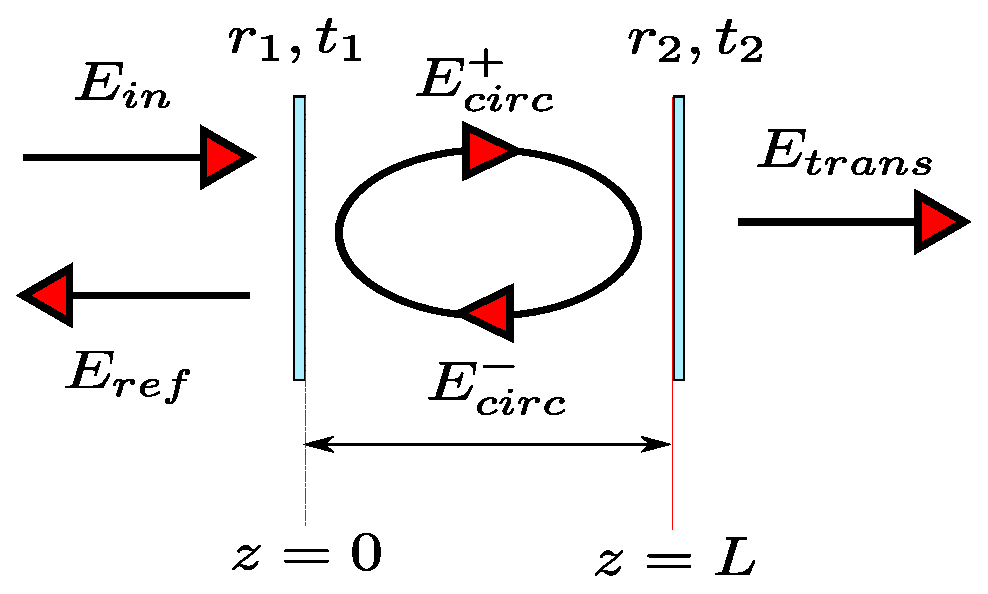
\includegraphics[scale=0.8]{E-field_model_edit.eps}
\caption{Fabry-Perot amplitude field analysis scheme, with input field $E_{in}$ onto the left mirror, cavity reflected field $E_{ref}$, intra-cavity fields $E_{circ}^{\pm}$ and cavity transmission $E_{trans}$. The cavity length is $L$ and $z = 0$ is placed at the inner surface of the incoupling mirror.}
\label{fig:E-field_model}
\end{figure}

We assume planar waves for the electric fields, where the index arrows shows propagation direction according to figure \ref{fig:E-field_model}

\begin{align}
E_{\rightarrow}(t, z) & = E_{\rightarrow}e^{i(\omega_l t + kz)} \\
E_{\leftarrow}(t, z) & = E_{\leftarrow}e^{i(\omega_l t - kz)}.
\end{align}
\noindent
It should be noted that the actual electric field is given by real part $\Re[E(z, t)]$, and that we omit the term $e^{i\omega_l t}$ in the calculations, since it drops out. We can then relate the input and output by a transfer matrix, keeping in mind that for a lossless mirror the matrix must be unitary

\begin{subequations}
\begin{align}
\begin{pmatrix}
E_{circ}^{+}(z = 0) \\
E_{ref}(z = 0)
\end{pmatrix}
 & =
\begin{pmatrix}
it_1 & r_1 \\
r_1 & it_1
\end{pmatrix} 
\begin{pmatrix}
E_{in}(z = 0) \\
E_{circ}^{-}(z = 0)
\end{pmatrix} \\
\begin{pmatrix}
E_{trans}(z = L) \\
E_{circ}^{-}(z = L)
\end{pmatrix}
 & =
\begin{pmatrix}
it_2 & r_2 \\
r_2 & it_2
\end{pmatrix}
\begin{pmatrix}
E_{circ}^{+}(z = L) \\
0
\end{pmatrix}.
\end{align}
\label{eq:E-field_transfer}
\end{subequations}
\noindent
This expression yields four coupled equations. Using that $E_{circ}^-$ in terms of $E_{circ}^+$ is $E_{circ}^- = r_2E_{circ}^+e^{2ikL}$ and taking the high-finesse limit $r_{1,2} \rightarrow -1$, we get the steady state solution for the circulating intra-cavity fields

\begin{equation}
E_{circ}^- = E_{circ}^+ = \frac{it_1 E_{in}}{1 - r_1r_2e^{2ikL}}.
\label{eq:high_finesse_approx}
\end{equation}
\noindent
The intra-cavity fields become equal in this limit and we can easily plot how the transmission through the cavity looks for different reflectivity coefficients of the mirrors, whilst keeping $r_1 = r_2$, see figure \ref{fig:trans_curve_finesse}.

\begin{figure}[H]
\centering
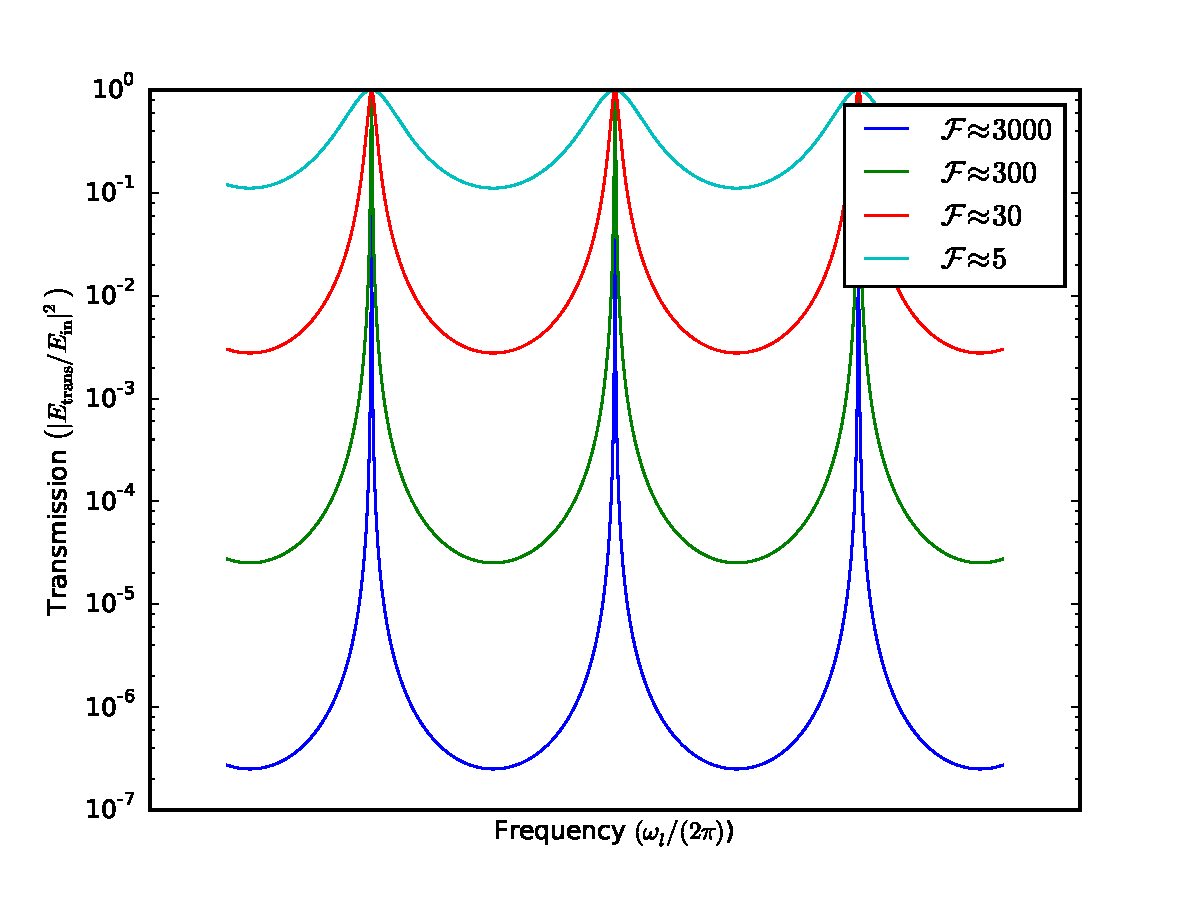
\includegraphics[scale=0.8]{cavity_model_fsr.pdf}
\caption{Transmissions through the cavity $\left| \frac{E_{trans}}{E_{in}} \right|^2$ whilst the laser frequency is changed for different finesses, i.e. reflection coefficients of the mirrors. Notice that the resonance peaks get broadened at lower finesse, this is due to an increase in $\kappa$, since it is the full-width-half-maximum of the lineshape. Another thing to notice is, that the spacing between each resonance corresponds to the $FSR$ of the cavity.}
\label{fig:trans_curve_finesse}
\end{figure}

%\begin{figure}[H]
%\centering
%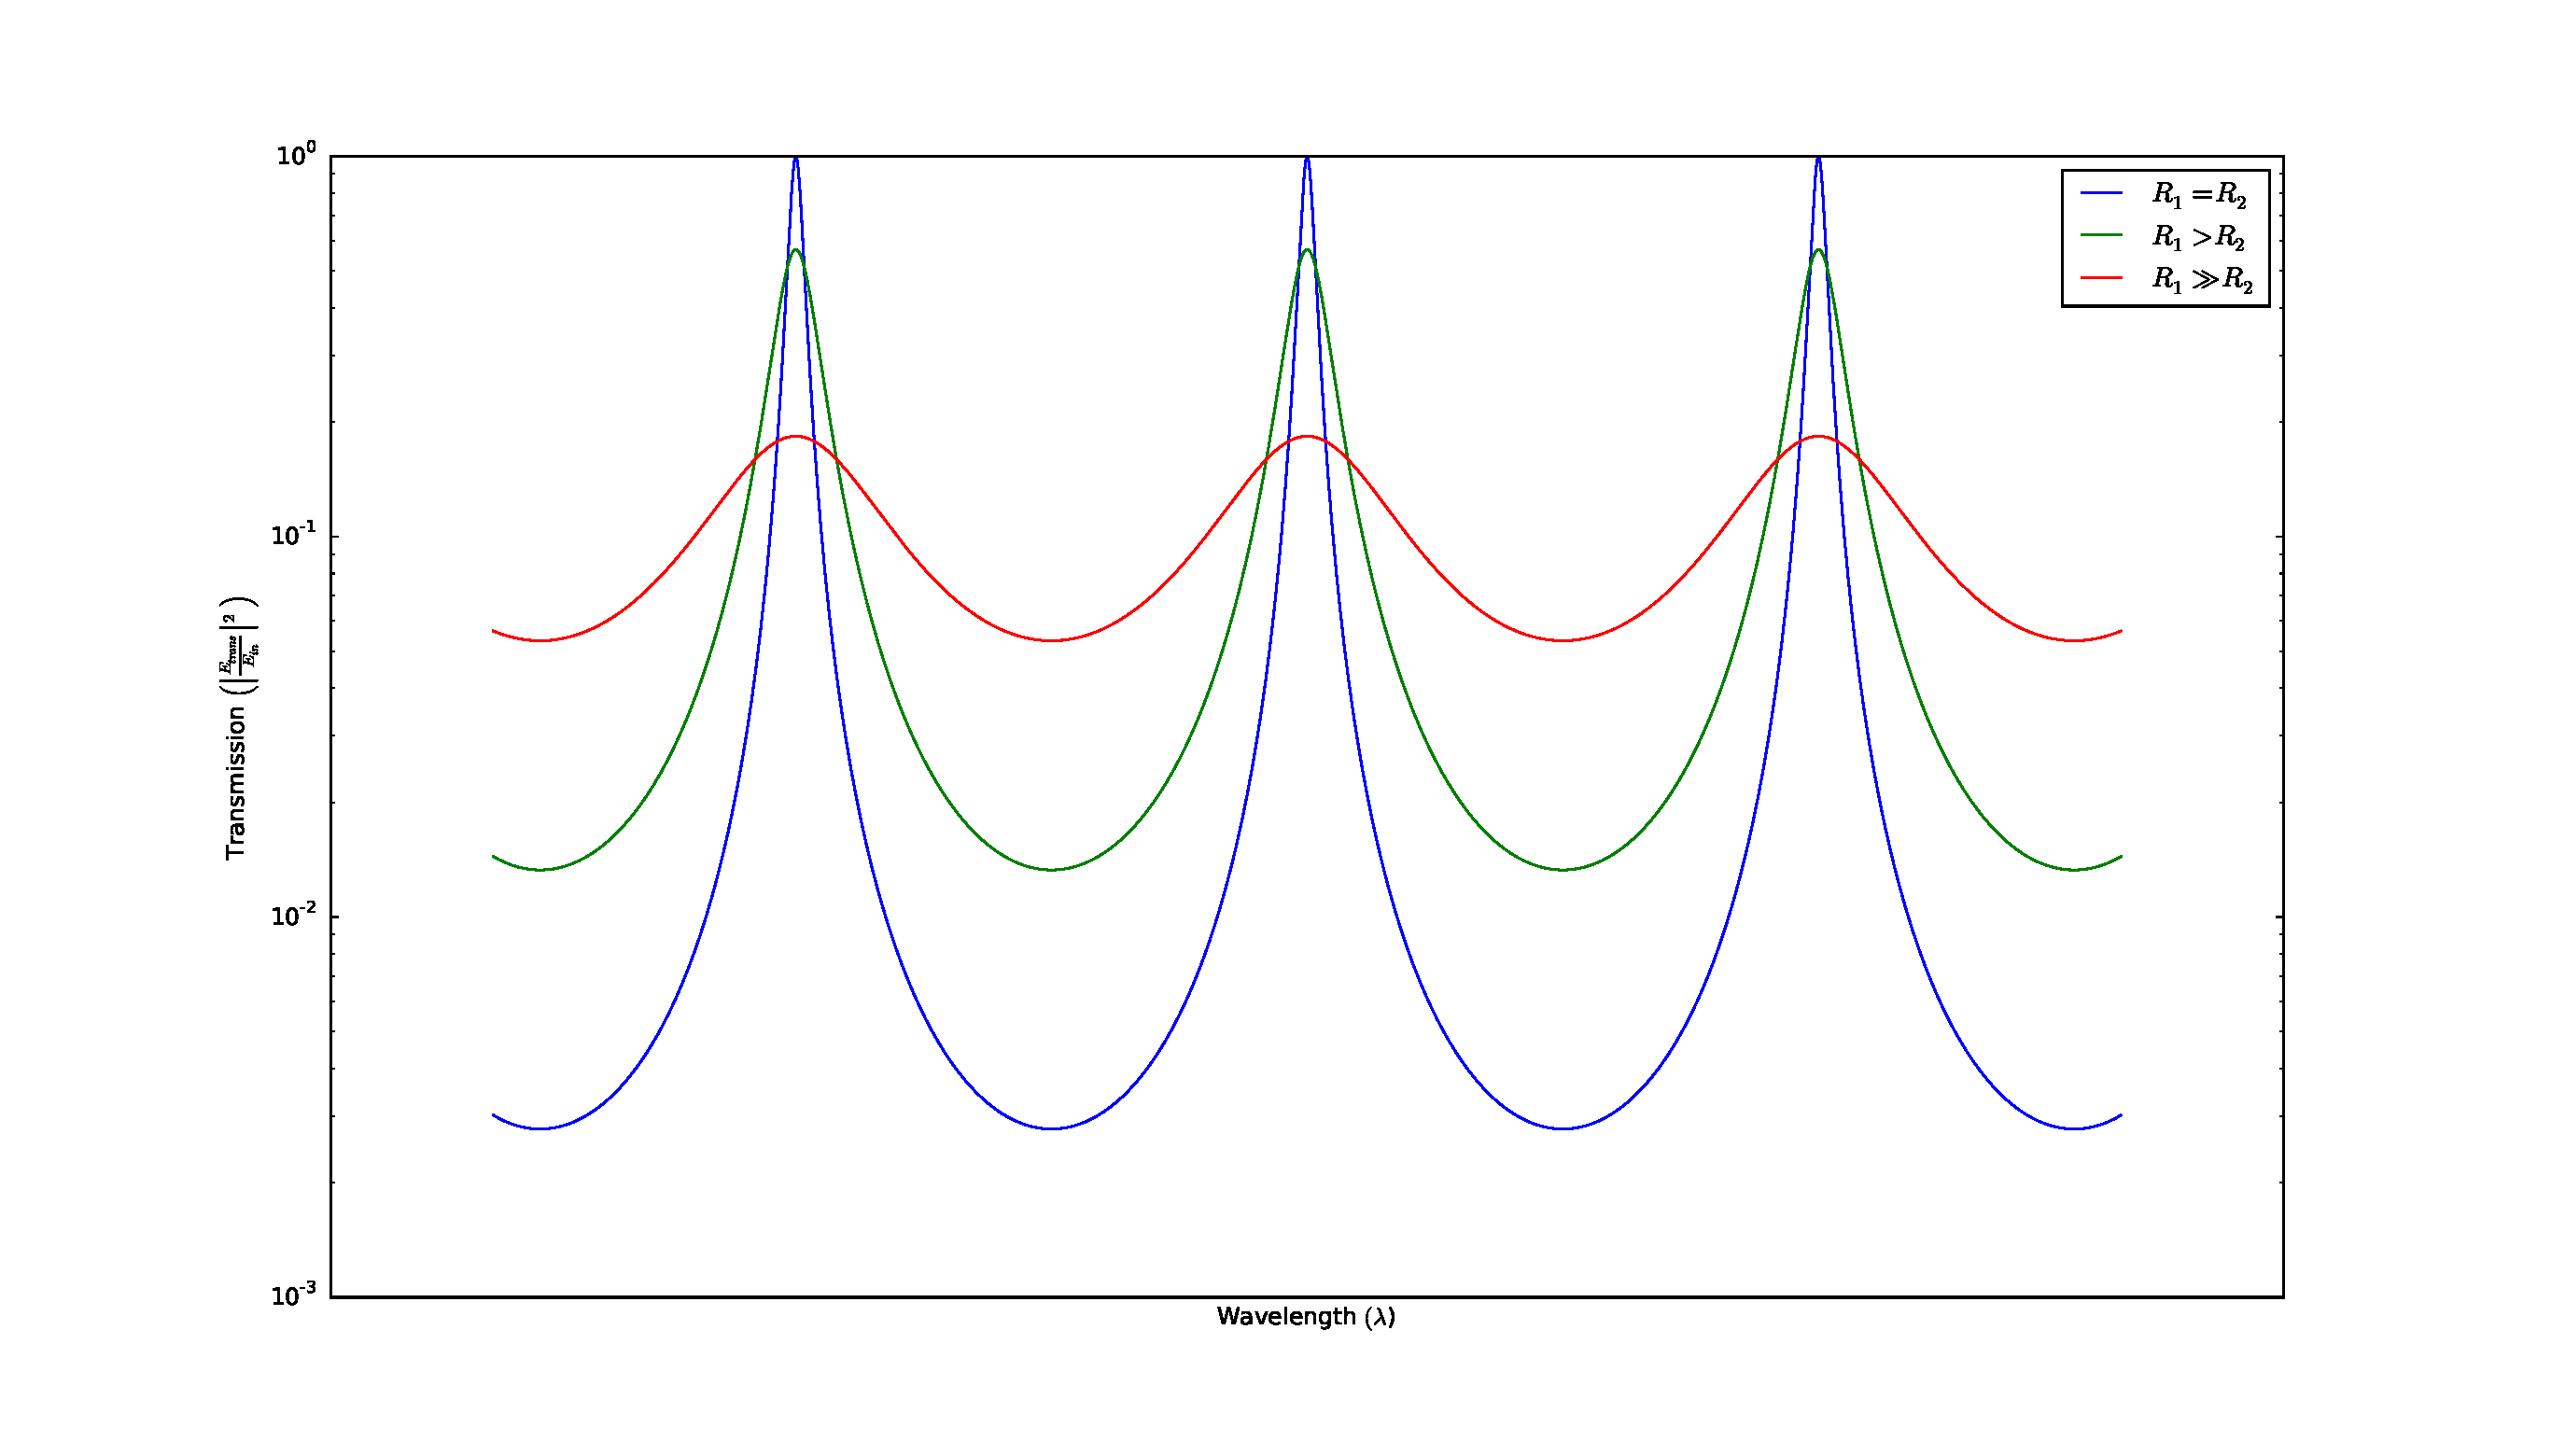
\includegraphics[scale=0.33]{trans_curve_reflections.eps}
%\caption{Bla bla}
%\label{fig:trans_curve_reflections}
%\end{figure}


We now depart from the steady state treatment and look at the slow build up and decay of the intra-cavity field. We allow for the amplitude of the fields to vary on a timescale much slower than the cavity round trip time $T_{rt} = \frac{2L}{c}$ the inverse of the free spectral range, and write

\begin{equation}
E_{circ}^+(t + T_{rt}) = it_1E_{in}(t) + r_1r_2e^{2ikL}E_{circ}^+(t),
\end{equation}
\noindent
where we have used the relation that the complex amplitude of a propagating field becomes multiplied by $r_1r_2e^{2ikL}$ after completing one round trip, thereby obtaining a relation for the time evolution of the circulating field: we obtain the differential equation

\begin{equation}
\frac{\mathrm{d}E_{circ}^+}{\mathrm{d}t} \approx \frac{E_{circ}^+(t + T_{rt}) - E_{circ}^+(t)}{T_{rt}} = \frac{it_1E_{in(t)}}{T_{rt}} + \left( r_1r_2e^{2ikL} - 1 \right)\frac{E_{circ}^+(t)}{T_{rt}}.
\label{eq:diff_field}
\end{equation}
\noindent
Previously we assumed high finesse limit to first order, but now we will include second order terms $r_1r_2 \approx 1 - (\frac{t_1^2}{2} + \frac{t_1^2}{2})$ and include low internal loss into the system. We model internal loss as a small imaginary component added to the regular wave number $k = \frac{\omega_L}{c}$:

\begin{equation}
e^{2ik'L} \approx \left(1 - \frac{\delta_{loss}}{2}\right)e^{2ikL}.
\end{equation}
\noindent
We now need to consider, what happens to the round trip phase $e^{2ikL}=e^{i\frac{\omega_L}{FSR}}$ close to cavity resonance $\omega_c$

\begin{equation}
e^{i\frac{\omega_L}{FSR}} \approx 1 - i\left( \frac{\omega_L - \omega_c}{FSR}\right).
\end{equation}
\noindent
We look back at equation \eqref{eq:high_finesse_approx} and remember that the magnitude of the intra-cavity fields traveling in both directions become equal in the high finesse limit. This means that the total circulating field $E_{circ}(t, z) = E_{circ}^{+}(t, z) + E_{circ}^{-}(t, z)$ becomes

\begin{equation}
E_{circ}(t, z) = 2E_{circ}(t)e^{i\omega_Lt}\sin(kz),
\end{equation}
\noindent
where $E_{circ}(t) \equiv iE_{circ}^+(t)$. We can now rewrite equation \eqref{eq:diff_field} in terms of $E_{circ}$ omitting second order terms

\begin{equation}
\frac{\mathrm{d}E_{circ}(t)}{\mathrm{d}t} \approx \frac{t_1E_{in}(t)}{T_{rt}} - E_{circ}(t)\left( \frac{t_1^2/2 + t_2^2/2 +\delta_{loss}/2}{T_{rt}} + i(\omega_L - \omega_c) \right).
\end{equation}
\noindent
This is basically the cavity equation of motion, but commonly we rescale the intra-cavity field with a factor of $E_{circ}(t)\sqrt{T_{rt}} = a(t)$. The newly defined variable is now normalized to the square root of the circulating intra-cavity energy; $a(t) = \sqrt{U_{circ}(t)}$, where the energy is related to the power by $U_{circ}(t) = T_{rt}P_{circ}(t)$. The rescaling is mainly done because the conversion to number of photons is easy, we just need to divide the energy with the energy of our photon $\hbar\omega_l$. Conversion to power, which we measure in the lab, is also easy. The equation of motion then reads

\begin{equation}
\dot{a}(t) = -\left(\frac{\kappa}{2} + i\Delta\right)a(t) + \sqrt{\kappa_1}E_{in}(t),
\label{eq:cavity_eom}
\end{equation}
\noindent
where the detuning is $\Delta = \omega_L - \omega_c$ and the sum of the decay rates is $\kappa = \kappa_1 + \kappa_2 + \kappa_{l}$, the transmission decay rates is $\kappa_{1,2} = \frac{t_{1,2}^2}{T_{rt}}$ and the internal loss rate is $\kappa_{l} = \frac{\delta_{loss}}{T_{rt}}$. We indentify the external losses $\kappa_{ex}$ with $\kappa_1$ and the rest with $\kappa_0$.